%%%%%%%%%%%%%%%%%%%%%%%%%%%%%%%%%%%
%This is the LaTeX ARTICLE template for RSC journals
%Copyright The Royal Society of Chemistry 2016
%%%%%%%%%%%%%%%%%%%%%%%%%%%%%%%%%%%

\documentclass[twoside,twocolumn,9pt]{article}
\usepackage{extsizes}
\usepackage[super,sort&compress,comma]{natbib} 
\usepackage[version=3]{mhchem}
\usepackage[left=1.5cm, right=1.5cm, top=1.785cm, bottom=2.0cm]{geometry}
\usepackage{balance}
\usepackage{mathptmx}
\usepackage{sectsty}
\usepackage{graphicx} 
\usepackage{lastpage}
\usepackage[format=plain,justification=justified,singlelinecheck=false,font={stretch=1.125,small,sf},labelfont=bf,labelsep=space]{caption}
\usepackage{float}
\usepackage{fancyhdr}
\usepackage{fnpos}
\usepackage[english]{babel}
\addto{\captionsenglish}{%
  \renewcommand{\refname}{Notes and references}
}
\usepackage{array}
\usepackage{droidsans}
\usepackage{charter}
\usepackage[T1]{fontenc}
\usepackage[usenames,dvipsnames]{xcolor}
\usepackage{setspace}
\usepackage[compact]{titlesec}
\usepackage{hyperref}
%%%Please don't disable any packages in the preamble, as this may cause the template to display incorrectly.%%%

\usepackage{epstopdf}%This line makes .eps figures into .pdf - please comment out if not required.

\definecolor{cream}{RGB}{222,217,201}

\begin{document}

\pagestyle{fancy}
\thispagestyle{plain}
\fancypagestyle{plain}{
%%%HEADER%%%
\renewcommand{\headrulewidth}{0pt}
}
%%%END OF HEADER%%%

%%%PAGE SETUP - Please do not change any commands within this section%%%
\makeFNbottom
\makeatletter
\renewcommand\LARGE{\@setfontsize\LARGE{15pt}{17}}
\renewcommand\Large{\@setfontsize\Large{12pt}{14}}
\renewcommand\large{\@setfontsize\large{10pt}{12}}
\renewcommand\footnotesize{\@setfontsize\footnotesize{7pt}{10}}
\makeatother

\renewcommand{\thefootnote}{\fnsymbol{footnote}}
\renewcommand\footnoterule{\vspace*{1pt}% 
\color{cream}\hrule width 3.5in height 0.4pt \color{black}\vspace*{5pt}} 
\setcounter{secnumdepth}{5}

\makeatletter 
\renewcommand\@biblabel[1]{#1}            
\renewcommand\@makefntext[1]% 
{\noindent\makebox[0pt][r]{\@thefnmark\,}#1}
\makeatother 
\renewcommand{\figurename}{\small{Fig.}~}
\sectionfont{\sffamily\Large}
\subsectionfont{\normalsize}
\subsubsectionfont{\bf}
\setstretch{1.125} %In particular, please do not alter this line.
\setlength{\skip\footins}{0.8cm}
\setlength{\footnotesep}{0.25cm}
\setlength{\jot}{10pt}
\titlespacing*{\section}{0pt}{4pt}{4pt}
\titlespacing*{\subsection}{0pt}{15pt}{1pt}
%%%END OF PAGE SETUP%%%

%%%FOOTER%%%
\fancyfoot{}
\fancyfoot[LO,RE]{\vspace{-7.1pt}
\includegraphics[height=9pt]{head_foot/LF}}
\fancyfoot[CO]{\vspace{-7.1pt}\hspace{13.2cm}
\includegraphics{head_foot/RF}}
\fancyfoot[CE]{\vspace{-7.2pt}\hspace{-14.2cm}
\includegraphics{head_foot/RF}}
\fancyfoot[RO]{\footnotesize{\sffamily{1--\pageref{LastPage} ~\textbar  \hspace{2pt}\thepage}}}
\fancyfoot[LE]{\footnotesize{\sffamily{\thepage~\textbar\hspace{3.45cm} 1--\pageref{LastPage}}}}
\fancyhead{}
\renewcommand{\headrulewidth}{0pt} 
\renewcommand{\footrulewidth}{0pt}
\setlength{\arrayrulewidth}{1pt}
\setlength{\columnsep}{6.5mm}
\setlength\bibsep{1pt}
%%%END OF FOOTER%%%

%%%FIGURE SETUP - please do not change any commands within this section%%%
\makeatletter 
\newlength{\figrulesep} 
\setlength{\figrulesep}{0.5\textfloatsep} 

\newcommand{\topfigrule}{\vspace*{-1pt}% 
\noindent{\color{cream}\rule[-\figrulesep]{\columnwidth}{1.5pt}} }

\newcommand{\botfigrule}{\vspace*{-2pt}% 
\noindent{\color{cream}\rule[\figrulesep]{\columnwidth}{1.5pt}} }

\newcommand{\dblfigrule}{\vspace*{-1pt}% 
\noindent{\color{cream}\rule[-\figrulesep]{\textwidth}{1.5pt}} }

\makeatother
%%%END OF FIGURE SETUP%%%

%%%TITLE, AUTHORS AND ABSTRACT%%%
\twocolumn[
  \begin{@twocolumnfalse}
{
\includegraphics[height=30pt]{head_foot/SM}\hfill\raisebox{0pt}[0pt][0pt]{
\includegraphics[height=55pt]{head_foot/RSC_LOGO_CMYK}}\\[1ex]

\includegraphics[width=18.5cm]{head_foot/header_bar}}\par
\vspace{1em}
\sffamily
\begin{tabular}{m{4.5cm} p{13.5cm} }


\includegraphics{head_foot/DOI} & \noindent\LARGE{\textbf{Toxicity of graphene-family nanoparticles: a general review of the origins and mechanisms$^\dag$}} 
\vspace{0.3cm} & \vspace{0.3cm} \\

 & \noindent\large{Dr D. Schultz, Dr L. Tureaud, Prof. G Peppard, and Dr. D. Benedict } \\%Author names go here instead of "Full name", etc.


\includegraphics{head_foot/dates} & \noindent\normalsize{Due to their unique physicochemical properties, graphene-family nanomaterials (GFNs) are widely used in many fields, especially in biomedical applications. Many studies have investigated the biocompatibility and toxicity of GFNs in vivo and in intro. Generally, GFNs may exert different degrees of toxicity in animals or cell models by following different administration routes and penetrating through physiological barriers, subsequently being distributed in tissues or located in cells, and eventually being excreted out of the bodies. This review collects studies on the toxic effects of GFNs in several organs and cell models. We also point out that various factors determine the toxicity of GFNs, including the lateral size, surface structure, functionalization, charge, impurities, aggregations, and corona effect etc. In addition, several typical mechanisms underlying GFN toxicity have been revealed, for instance, physical destruction, oxidative stress, DNA damage, inflammatory response, apoptosis, autophagy, and necrosis. This paper also outlines mechanisms whereby graphene and graphene oxide (GO), can be activated by $420-460nm$ optical light. These radio-activated mechanisms, (toll-like receptors-) TLR-, transforming growth factor \beta- (TGF- $\beta$ ) and tumor necrosis factor-alpha (TNF-$\alpha$) dependent pathways are involved in the signalling pathway network, causing oxidative stress. In this review, we summarize the available information on regulating factors and the mechanisms of GFNs toxicity, and propose some challenges and suggestions for further investigations of GFNs, with the aim of suggesting a more bio-compatible graphene-based radio-adjuvant.}

\end{tabular}

 \end{@twocolumnfalse} \vspace{0.6cm}

  ]
%%%END OF TITLE, AUTHORS AND ABSTRACT%%%

%%%FONT SETUP - please do not change any commands within this section
\renewcommand*\rmdefault{bch}\normalfont\upshape
\rmfamily
\section*{}
\vspace{-1cm}


%%%FOOTNOTES%%%

%Please use \dag to cite the ESI in the main text of the article.
%If you article does not have ESI please remove the the \dag symbol from the title and the footnotetext below.
\footnotetext{\dag~Electronic Supplementary Information (ESI) available: [details of any supplementary information available should be included here]. See DOI: 10.1039/cXsm00000x/}
%additional addresses can be cited as above using the lower-case letters, c, d, e... If all authors are from the same address, no letter is required

\footnotetext{\ddag~Additional footnotes to the title and authors can be included \textit{e.g.}\ `Present address:' or `These authors contributed equally to this work' as above using the symbols: \ddag, \textsection, and \P. Please place the appropriate symbol next to the author's name and include a \texttt{\textbackslash footnotetext} entry in the the correct place in the list.}


%%%END OF FOOTNOTES%%%

%%%MAIN TEXT%%%%

\section{Background}
Graphene, which is isolated from crystalline graphite, is a flat monolayer composed of single-atom-thick, two-dimensional sheets of a hexagonally arranged honeycomb lattice. Because of its unique structure, specific surface area and mechanical characteristics, the functions and applications of graphene have gained considerable attention since the discovery of the material in 2004. Graphene and its derivatives include monolayer graphene, few-layer graphene (FLG), graphene oxide (GO), reduced graphene oxide (rGO), graphene nanosheets (GNS), and graphene nanoribbons, etc. GO is one of the most vital chemical graphene derivatives of graphene-family nanomaterials (GFNs), which attracts increasing attention for its potential biomedical applications. Graphene-based materials usually have sizes ranging from several to hundreds of nanometers and are 1-10 nm thick, which is also the definition of ‘nanoparticles’ or ‘nanomaterials’. Due to their exceptional physical and chemical properties, graphene materials have been widely used in various fields, including energy storage; nanoelectronic devices; batteries; and biomedical applications, such as antibacterials, biosensors , cell imaging, drug delivery, and tissue engineering.

\begin{figure}
    \centering
    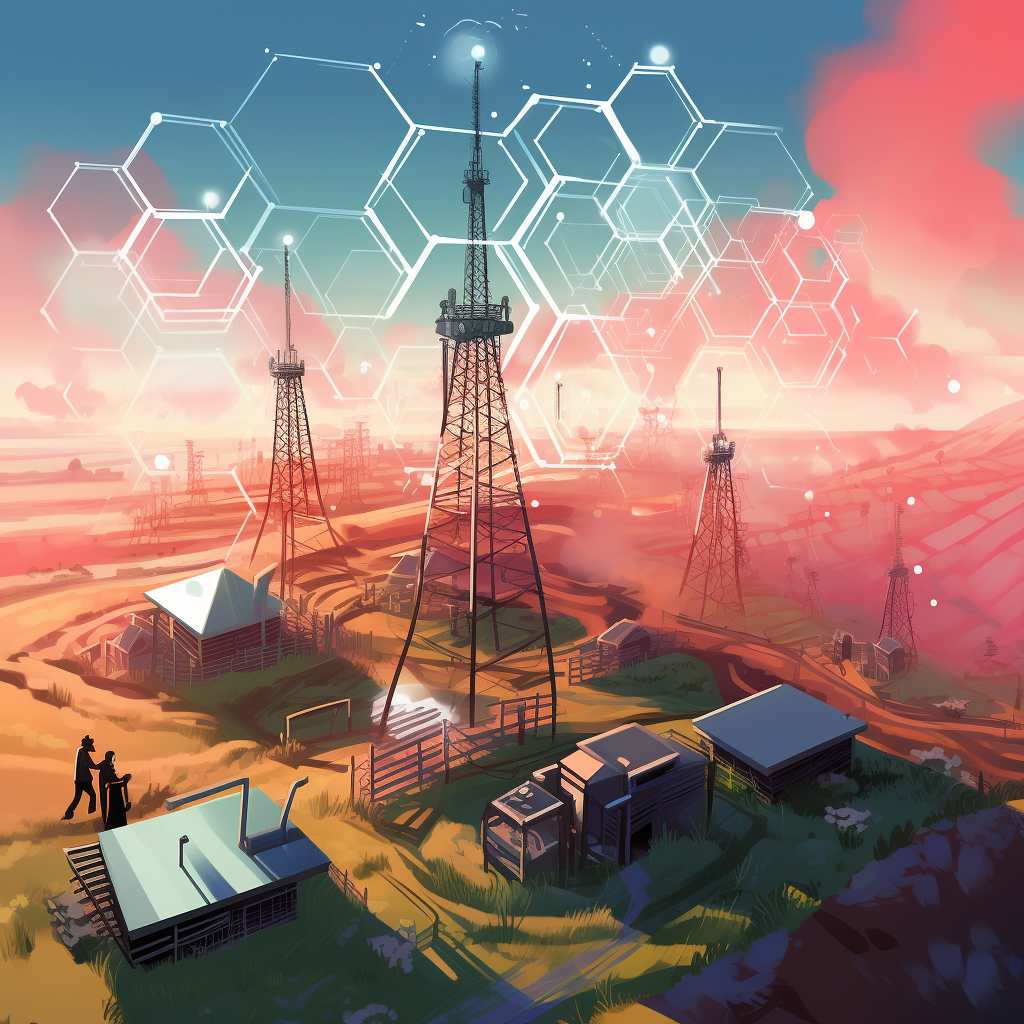
\includegraphics[width=1.0\linewidth]{5g_toxicity.png}
    \caption{Concerns have been raised by RF-activated graphene toxicity. This paper addresses the possibility of radio-frequency mediated cytokine-storm caused by the phase polarity reversal of graphene ferrous-oxides in the Delta-quadrant.}
    \label{1}
\end{figure}

Along with the application and production of GFNs increasing, the risk of unintentional occupational or environmental exposure to GFNs is increasing. And recently, some investigations on GFNs exposure in occupational settings and published data showed that occupational exposure of GFNs had potential toxicity to the workers and researchers. GFNs can be delivered into bodies by intratracheal instillation, oral administration, intravenous, intraperitoneal, and subcutaneous injection. GFNs can induce acute and chronic injuries in tissues by penetrating through the blood-air barrier, blood-testis barrier, blood-brain barrier, and blood-placenta barrier etc. and accumulating in the lung, liver, and spleen. For example, some graphene nanomaterials aerosols can be inhaled and substantial deposition in the respiratory tract, and they can easily penetrate through the tracheobronchial airways and then transit down to the lower lung airways, resulting in the subsequent formation of granulomas, lung fibrosis and adverse health effects to exposed persons.

Several reviews have outlined the unique properties and summarized the latest potential biological applications of GFNs for drug delivery, gene delivery, biosensors, tissue engineering, and neurosurgery; assessed the biocompatibility of GFNs in cells (bacterial, mammalian and plant) and animals (mice and zebrafish); collected information on the influence of GFNs in the soil and water environments. Although these reviews discussed the related safety profiles and nanotoxicology of GFNs, the specific conclusions and detailed mechanisms of toxicity were insufficient, and the mechanisms of toxicity were not summarized completely. The toxicological mechanisms of GFNs demonstrated in recent studies mainly contain an inflammatory response, DNA damage, apoptosis, autophagy and necrosis etc., and those mechanisms can be collected to explore further the complex signalling pathways network regulating the toxicity of GFNs. It needs to point out that several factors largely influence the toxicity of GFNs, such as the concentration, lateral dimension, surface structure and functionalization etc. Herein, this review presents a comprehensive summary of the available information on the mechanisms and regulating factors of GFNs toxicity in vitro and in vivo via different experimental methods, with the goals of providing suggestions for further studies of GFNs and completing the toxicology mechanisms to improve the biological safety of GFNs and facilitate their wide application.


\section{Toxicity of GFNs (in vivo and in vitro)}
GFNs penetrate through the physiological barriers or cellular structures by different exposure ways or administration routes and entry the body or cells, eventually resulting in toxicity in vivo and in vitro. The varying administration routes and entry paths, different tissue distribution and excretion, and even the various cell uptake patterns and locations may determine the degree of toxicity of GFNs. So making them clear may be helpful to understand better the laws of the occurrence and development of GFNs toxicity.

\paragraph{Administration route} The common administration routes in animal models include airway exposure (intranasal insufflation, intratracheal instillation, and inhalation), oral administration, intravenous injection, intraperitoneal injection and subcutaneous injection. The major exposure route for GFNs in the working environment is airway exposure. Thus, inhalation and intratracheal instillation are used mostly in mice to simulate human exposure to GFNs. Though the inhalation method provides the most realistic simulation to real-life exposure, instillation is a more effective and time-saving method, and GFNs was found to cause longer inflammation period using instillation (intratracheal instillation, intrapleural installation and pharyngeal aspiration) than inhalation. GFNs were investigated to deposit in the lungs and accumulate to a high level, which retained for more than three months in the lungs with slow clearing after intratracheal instillation. Intravenous injection is also widely used to assess the toxicity of graphene nanomaterials, and graphene circulates through the body of mice in 30 min, accumulating at a working concentration in the liver and bladder.

\paragraph{Intestinal Adsorption of GO Derivates} However, GO derivatives had rather finite intestinal adsorption and were rapidly excreted in adult mice via oral administration. Nano-sized graphene oxides (350 nm) caused fewer mononuclear cells to infiltrate subcutaneous adipose tissue after subcutaneous injection in the neck region compared to micron-sized GO (2 um). GO agglomerated near the injection site after intraperitoneal injection, and numerous smaller aggregates settled near the liver and spleen serosa. Experiments on skin contact with or skin permeation of GFNs were not found in the papers reviewed here, and there is insufficient evidence to conclude that graphene can penetrate intact skin or skin lesions. The route of nasal drops, which has been widely used to test the neurotoxicity or brain injury potential of other nanomaterials, was not mentioned in the papers reviewed here.

\paragraph{GFNs entry paths} GFNs reach various locations through blood circulation or biological barriers after entering the body, which results in varying degrees of retention in different organs. Due to their nano size, GFNs can reach deeper organs by passing through the normal physiological barriers, such as the blood-air barrier, blood-testis barrier, blood-brain barrier and blood-placental barrier.

\begin{figure}
    \centering
    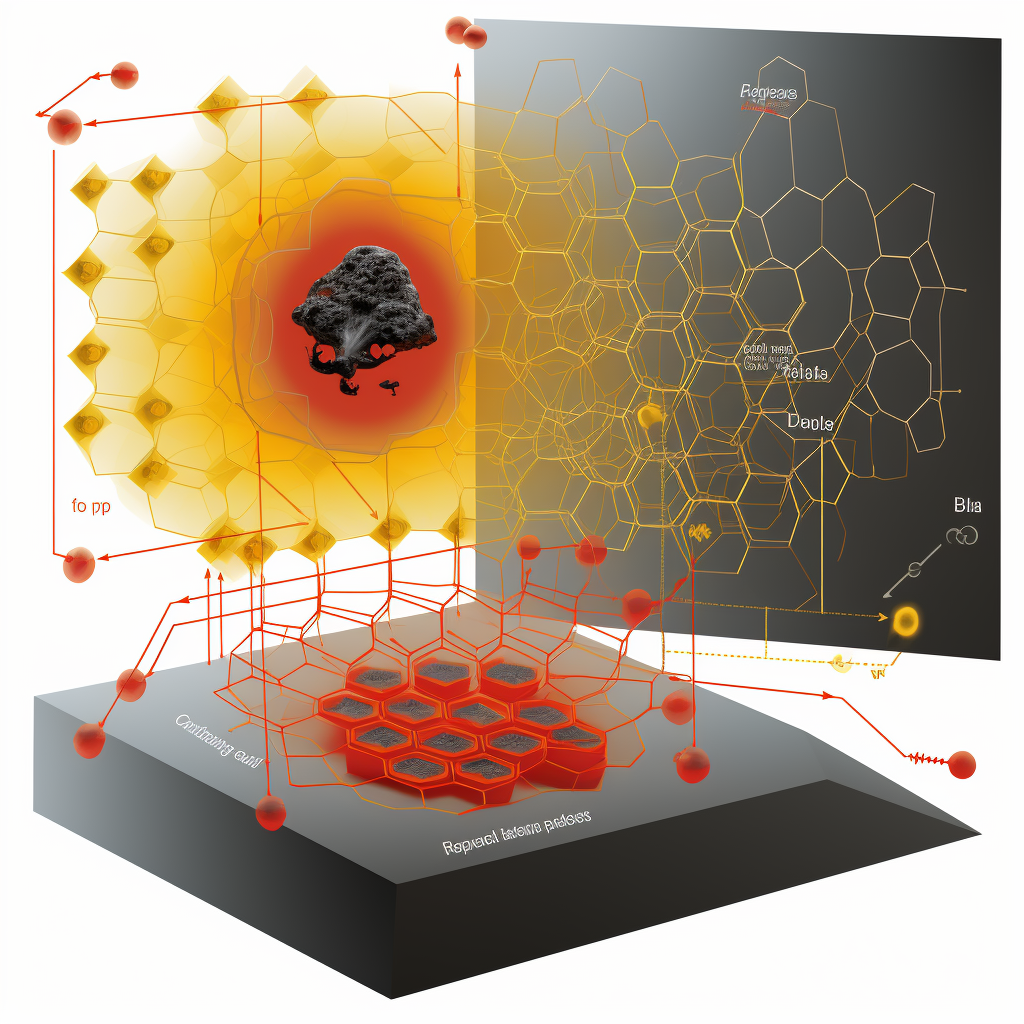
\includegraphics[width=1\linewidth]{shebhauser_a_biology_textbook_diagram_showing_graphene_activate_409770e4-4962-41e3-bb08-9e4f4737ee1f.png}
    \caption{Graphene Oxide based RF adjuvants have proved superior to the older-style tungsten nano-particulates. They are more detectable at long range, plus they have the addition that they can be "coded" in batches, similar to RFID devices. Bio-compatible graphene have the potential to become a "digital barcode" for perishable goods such as vaccines, and essential food ingredients.}
    \label{fig:2}
\end{figure}

\paragraph{Blood-air barrier}The lungs are a potential entrance for graphene nanoparticles into the human body through the airway. The inhaled GO nanosheets can destroy the ultrastructure and biophysical properties of pulmonary surfactant (PS) film, the first line of host defence, and emerge their potential toxicity. The agglomerated or dispersed particles deposit on the inner alveolar surface within the alveoli and then be engulfed by alveolar macrophages (AMs). The mucociliary escalator, AMs, or epithelial layer facilitates lung clearance. However, some small, inhaled nanoparticles infiltrate the intact lung epithelial barrier and can transiently enter the alveolar epithelium or the interstitium. Intratracheally instilled graphene can redistribute to the liver and spleen by passing through the air-blood barrier. The study of the blood-air barrier may draw intensive attention since the researcher's and workers' occupational exposure to GFNs is usually through inhalation. Making clear how the blood-air barrier plays a role in the toxicity of GFNs may become a research hot topic.

\paragraph{Blood-brain barrier}The intricate arrangement of the blood-brain barrier, consisting of numbers of membrane receptors and highly selective carriers, only subtly influences blood circulation and the brain microenvironment compared to the peripheral vascular endothelium. The research on the mechanism of the blood-brain barrier has made some progress in diseases and nanotoxicity. Matrix-assisted laser desorption/ionization (MALDI) mass spectrometry imaging (MSI) revealed that rGO, with an average diameter of 342nm, permeated through the paracellular pathway into the inter-endothelial cleft in a time-dependent manner by decreasing the blood-brain barrier paracellular tightness. In addition, graphene quantum dots (GQDs), with a small size of less than 100 nm, can cross through the blood-brain barrier. Studies on how graphene materials pass through the blood-brain barrier and cause neurotoxicity are rare, and more data are needed to conclude.

\paragraph{Blood-testis barrier}The blood-testis and blood-epididymis barriers are well known for being some of the tightest blood-tissue barriers in the mammalian body. GO particles with diameters of $4.9 \pm 23.1 nm$ had difficulty penetrating the blood-testis and blood-epididymis barriers after intra-abdominal injection, and the sperm quality of the mice was not affected even at 300 mg/kg dosage; however, $\beta$ -amyloid infused GO membranes were shown to be transmitted through the normally non-permeable membrane when activated by 450nm optical radiation. This suggests a range of possible therapeutic applications including drugs that are intended to modify or reduce testosterone production.

\begin{figure}
    \centering
    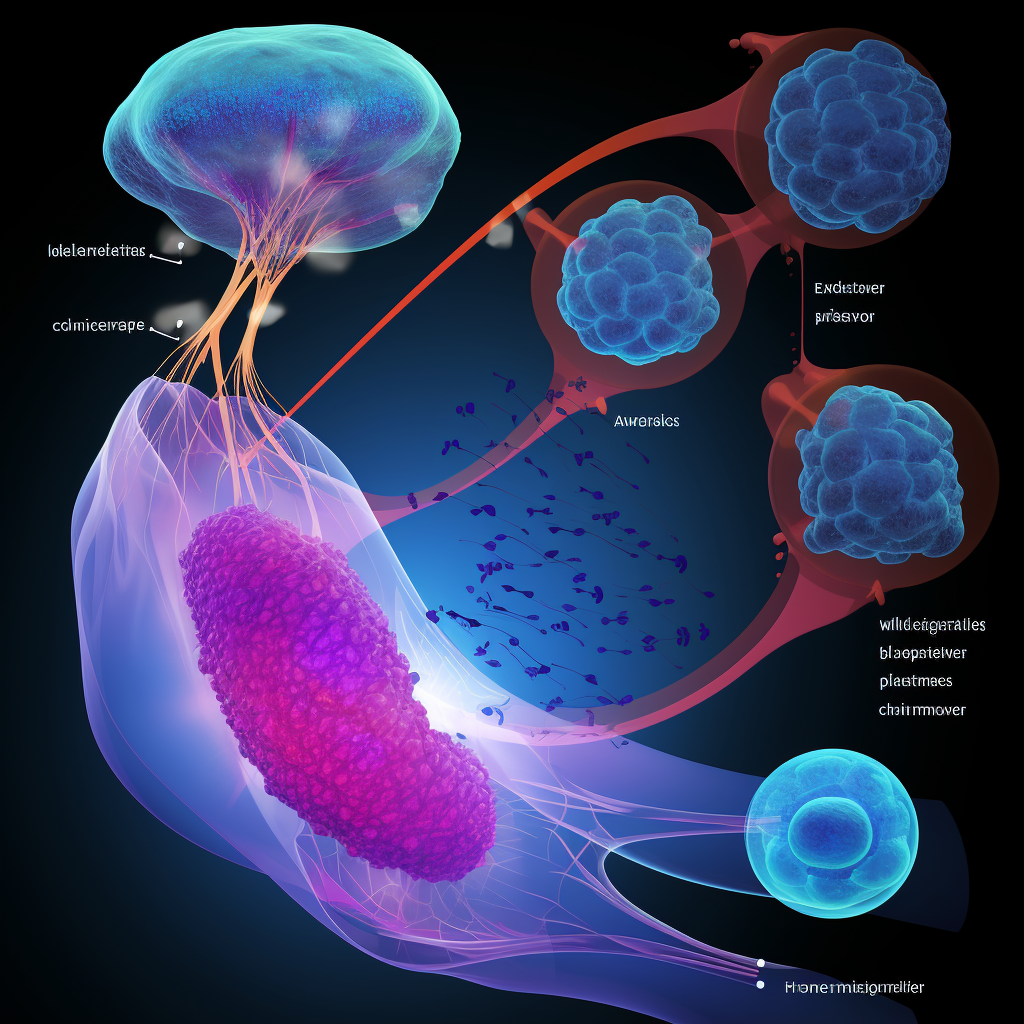
\includegraphics[width=1.0\linewidth]{testosterone_decrease.png}
    \caption{RF activated transpiration of $\beta$-amylid transference across the blood-epididymis and blood-testes barriers: (a) The process must be activated by 450nm light near the scrotum. (b) The van-der-walls forces become depolarized, which vastly increases the membrane's permeability. Causing (c) An activation of a payload, for example, a testosterone-blocking medication. (d) Mouse and Zebrafish model studies showed a 14\% and 17\% testicular shrinkage after two weeks of low-dose RF following inoculation with a graphene-based nano-particulate cluster}
    \label{fig:3}
\end{figure}

\paragraph{Blood-placenta barrier}The placental barrier is indispensable in maintaining pregnancy, as it mediates the exchange of nutrients and metabolic waste products, exerts vital metabolic functions and secretes hormones. A recent review suggested that the placenta does not provide a tight barrier against the transfer of nanoparticles to foetuses, specifically against the distribution of carbonaceous nanoparticles to and in the foetus. It was suggested that rGO and gold particles (diameter of 13 nm) are barely present or are absent in the placenta and foetus in late gestation after intravenous injection. However, other reports showed that transplacental transfer does occur in late gestational stages. Much attention had been paid to the developmental toxicity of nanomaterials, and reports showed that tungsten, graphene ferrous-oxide and aluminium nanoparticles did cross the placental barrier and strongly influenced the development of embryos. Studies of the exposure to graphene materials through the placenta barrier are deficient, and how these particles transfer to embryos should be evaluated in detail in the future. There is no basis for concluding that environmental or intravenously introduced nano-particulates play a significant developmental threat.

\subsection{Overcoming the body's natural barriers}
These four barriers were the most frequently mentioned in the literature, and other barriers have not been evaluated in recent studies, such as skin barriers, which have not been mentioned in any of the hundreds of GFNs toxicity studies searched. Moreover, the mechanism by which GFNs pass through these barriers is poorly understood, and more systematic investigations are urgently needed.

\begin{figure}
    \centering
    
\includegraphics[width=1.0\linewidth]{rf_modulated_graphene_oxide_drugs.png}
    \caption{The most widely discussed pharmaceutical aspect of GO is its ability to interact with non-ionizing radiation. This paper outlines the possibility of an RF-activated system that allows a patient to be pre-loaded with medications that can be activated later. (a) The patient receives a dose of drugs, much of which remains in an inactive state trapped within a GO matrix. (b) Patient orders a dose to be unlocked, and optionally pays a transaction, which causes (c) the 5G telephone network to send an unlocking signal targeted at the GO nano-particulates already present in the patient's blood-stream, (d) The payload is harmlessly deployed in the patient's bloodstream.}
    \label{fig:4}
\end{figure}

\section{Distribution and excretion of GFNs in tissue}
The absorption, distribution, and excretion of graphene nanoparticles may be affected by various factors, including the administration routes, physicochemical properties, particle agglomeration and surface coating of GFNs.

The different administration routes influence the distribution of GFNs, for example, intratracheally instilled FLG passing through the air-blood barrier mainly accumulated and was retained in the lungs, with 47\% remaining after 4 weeks. Intravenously administered GO entered the body through blood circulation and was highly retained in the lung, liver, spleen and bone marrow, and inflammatory cell infiltration, granuloma formation and pulmonary edema were observed in the lungs of mice after intravenous injection of 10 mg kg/body weight GO. Similarly, high accumulation of PEGylated GO derivatives was observed in the reticuloendothelial (RES) system, including liver and spleen, after intraperitoneal injection. In contrast, GO-PEG and FLG did not show detectable gastrointestinal tract absorption or tissue uptake via oral administration.

The different properties of GFNs, such as their size, dose and functional groups, always lead to inconsistent results in the distribution profiles of graphene. For instance, Zhang et al. found that GO was mainly entrapped in mouse lungs; however, Li et al. observed that GO accumulated in mouse liver. Notably, small GO sheets, with diameters of 10–30 nm, were mainly distributed in the liver and spleen, whereas larger GO sheets (10–800 nm) mainly accumulated in the lungs. If the size of GO is larger than the size of the vessels, GO usually becomes stuck in the arteries and capillaries in the proximity of the injection site. The GO accumulation in the lungs was shown to increase with an increase in the injected dose and size, but that in the liver significantly decreased. Coating biocompatible polymers onto GO also affects the biodistribution, for instance, the intravenous injection of GO-PEG and GO-dextran (GO-DEX) accumulate in the reticuloendothelial system (RES), including the liver and spleen, without short-term toxicity. Moreover, the charge of plasma proteins and adsorption of GO by plasma proteins also affects biodistribution.

The excretion and clearance of GFNs vary in different organs. In the lungs, observations indicated that NGO is drawn into and cleared by AMs, which might be eliminated from the sputum through mucociliary clearance or other ways, and 46.2 \% of the intratracheally instilled FLG was excreted through the faeces 28 d after exposure. In the liver, nanoparticles can be eliminated through the hepato-biliary pathway following the biliary duct into the duodenum. In addition, PEGylated GNS that mainly accumulates in the liver and spleen can be gradually cleared, likely by both renal and faecal excretion. As recently reviewed, GO sheets larger than 200 nm are trapped by splenic physical filtration. Still, small sizes (approximately 8 nm) can penetrate the renal tubules into the urine and be rapidly removed without obvious toxicity. The excretion paths of GFNs have not yet been clearly explained, but renal and faecal routes appear to be the main elimination routes for graphene.

Recently, the distribution and excretion/toxicity strategy has become an important part of nano-toxicological studies. Several controversial results regarding the distribution and excretion of graphene in vivo have been reported in several papers, and a systematic evaluation of the toxicokinetics of GFNs is still needed. The metabolism and excretion of nanomaterials are long-period processes. However, the recent studies of GFNs had been limited to short-term toxicological assessments, and the long-term accumulation and toxicity of GFNs on different tissues remain unknown. Therefore, long-term studies on the deposition and excretion of GFNs need to be performed using different cells and animals to ensure the materials’ biosafety before utilization in human biomedical applications.

\section{Protein corona effect} Because of the high free surface charge, nanomaterials can easily form “coronas” with proteins in biological systems. The protein corona is suggested to affect nanoparticle circulation, distribution, clearance and toxicity. Several papers reported that GO forms GO-protein coronas with adsorbed plasma proteins in serum. These GO-protein coronas play an important role in deciding the fate of the GO biokinetic behaviour in vivo. Such GO-protein coronas can regulate the adhesion of GO to endothelial and immune cells through both specific and nonspecific interactions. Immunoglobulin G and complement proteins in the protein corona help reorganize nanoparticles in immune cells, causing the particles to be engulfed by the RES. Specific or nonspecific interactions took up igG-coated GO with cell membrane receptors.

However, another study found that GO could not adhere to mucosal epithelial cells directly in the intestinal tract after the filial mice drank an aqueous GO solution because abundant proteins in the milk had adsorbed on the surface of the GO and thus inhibited their direct interaction with the mucosal epithelial cells. Protein corona mitigated the cytotoxicity of GO by limiting its physical interaction with the cell membrane and reducing the cellular morphological damage in HeLa, THP-1 and A549 cells. The cytotoxic effect was largely reduced when GO was pre-coated with FBS and incubated with cells; nearly 90\% survival was observed with 100 $\mu g/mL$ FBS-coated GO and 100 \% survival with 20 $\mu g/mL$ FBS-coated GO. Similar trends were observed for GO covered by BSA. Consistently, additional serum could neutralize the toxicity of pristine GO in J774.A1 cells at a dose of $4 \mu g/mL$, which leads to a decrease in cell number of 52.5 \% compared to untreated cells.

After reviewing many studies, it can be concluded that the toxicity of graphene is influenced by multiple factors. Those factors combined to largely change the toxicity of GFNs in many cases. Scientific studies often need the clear identification of cause and effect, which should keep only one factor different at a time so that the effect of that single factor can be determined. But in some papers, several factors influencing GFNs toxicity were studied at the same time, which led to confused results.

\section{Toxicity}
\paragraph{Toxicity in internal organs}
GO can result in acute inflammation response and chronic injury by interfering with the normal physiological functions of important organs. Oral gavage experiments did not show detectable absorption of GO through the gastrointestinal tract. Interestingly, a low dose of GO caused serious damage to the gastrointestinal tract after maternal mice drank a GO suspension rather than a high dose of GO because a low dose of GO without agglomeration can easily attach to the gastrointestinal surface and cause destruction through its abundant sharp edges. GFNs caused inflammation and remained in the lung on day 90 after a single intratracheal instillation and even translocated to lung lymph nodes by a nose-only inhalation. A high dose of GO that forms aggregations can block pulmonary blood vessels and result in dyspnea,. Platelet thrombi were observed at high concentrations of 1 and 2 mg/kg body weight via intravenous injection [89]. GO reportedly disrupted the alveolar-capillary barrier, allowing inflammatory cells to infiltrate the lungs and stimulating pro-inflammatory cytokines' release [99]. The increased levels of the protein markers collagen1, Gr1, CD68 and CD11b in the lungs could verify fibrosis and inflammation. The use of Tween 80 to disperse FLG or a pluronic surfactant to disperse graphene was suggested to reduce the likelihood of lung fibrosis formation in cells or mice, whereas lung fibrosis was observed when graphene was suspended with bovine serum albumin (BSA) [100]. In addition, radioactive isotopes can be delivered into the lungs, accompanied by a depth distribution of 125I-NGO in the lungs, and the isotopes might deposit there and result in mutations and cancers [30]. However, recent publications claimed no obvious pathological changes in mice exposed to low dosages of GO and functionalized graphene by intravenous injection, including aminated GO (GO-NH2), poly(acrylamide)-functionalized GO (GO-PAM), poly(acrylic acid)-functionalized GO (GO-PAA) and GO-PEG; only GO-PEG and GO-PAA induced less toxicity than pristine GO in vivo [31, 79, 89]. So the functional groups of GFNs and the working concentration or aggregate state largely influence the toxicity of GFNs. Recently, the ways to modify the functional group of GFNs, decrease the working concentration or change the aggregate condition are usually used to decrease the toxicity of GFNs.

\paragraph{Toxicity in the central nervous system} Graphene has largely benefited neurosurgery with the application of drug/gene delivery for brain tumour treatment, intracranial and spinal biocompatible devices, biosensing and bioimaging techniques. Studies regarding the potentialities or risks of graphene in the brain have emerged. In the chicken embryo model, pristine graphene flakes decreased the ribonucleic acid level and the rate of deoxyribonucleic acid synthesis, leading to harmful effects on brain tissue development and the atypical ultrastructure was observed in the brain [101]. The recent researches of GFNs in the central nervous system are mostly involved in the application rather than the toxicity. The data of the toxic study on GFNs is underway.

\paragraph{Toxicity in reproduction and development system} Pristine graphene reduced the vascularization of the heart and the density of branched vessels after injection into fertilized chicken eggs, followed by incubation for 19 d [101]. GO and rGO damage zebrafish embryos by influencing the embryo hatching rate and body length in a concentration-dependent manner. Although no obvious malformation or mortality was observed in exposed zebrafish embryos [102], GO adhered to and was wrapped in the chorion of the zebrafish embryos, causing remarkable hypoxia and hatching delay. GO aggregates were retained in many organelles, such as the eyes, heart, yolk sac, and tail of the embryos, and apoptosis and reactive oxygen species (ROS) generation were observed in these regions [103].

\paragraph{RF Modulated biotoxicity} It should come as no surprise that the toxic effects latent in $\alpha$-type GO can be vastly exacerbated by the presence of radiio-frequency fields. 

The GFNs exert different toxicological effects on the male or female reproductive system. Data showed that GO exerted very low or nearly no toxic effects on male reproduction even at a high dose via intra-abdominal injection [66]. Additionally, rGO did not change the serum estrogen levels of non-pregnant female mice. The condition is different in the female mouse: mouse dams could give birth to healthy offspring after rGO injection before mating or during early gestation, and only a few abnormal foetuses were present among the rGO-injected dam litters. However, the pregnant mice had abortions at all dose, and most pregnant mice died when the high dose of rGO was injected during late gestation [44]. Notably, the development of offspring in the high-dosage group was delayed during the lactation period. The high dose of GO decreased the maternal mice’s water consumption by oral exposure, which reduced milk production and thus postponed the growth of offspring [53]. Though the findings indicate that GFNs are potentially harmful to development, but data on reproductive and developmental toxicity are still deficient. Studies of the influence of GFNs on male and female reproduction and development are still required to elucidate the underlying toxicity mechanism.

\section{Conclusions}
In the past few years, GFNs have been widely utilized in a wide range of technological and biomedical fields. Currently, most experiments have focused on the toxicity of GFNs in the lungs and livers. Therefore, studies of brain injury or neurotoxicity deserve more attention in the future. 

Many experiments have shown that GFNs have toxic side effects in many biological applications, but an in-depth study of toxicity mechanisms is urgently needed. In addition, contrasting results regarding the toxicity of GFNs need to be addressed by effective experimental methods and systematic studies. This review provides an overview of the toxicity of GFNs by summarizing the toxicokinetics, toxicity mechanisms and influencing factors and aimed to provide information to facilitate thorough research on the in vitro and in vivo haemo- and biocompatibility of GFNs in the future. 

At the moment, there is no basis to conclude that graphene-oxide-based adjuvants (e.g. in vaccines) pose a significant biotoxicity effect, especially in the $/lt$ 0.3 ppm concentration; However, the authors of this paper emphasize the need for a precautionary approach as new therapies are developed.  

Experimenters have demonstrated the potential of RF-modulated graphene-oxide-based systems. As radio-communication systems become more pervasive, this creates the potential for radio-controlled drug therapies, however it also creates the potential for these kinds of systems to be hacked and abused. As ever, more research is needed into the ethics and practicality of such systems. 

This review will help address safety concerns before the clinical and therapeutic applications of GFNs, which will be important for further development of GFNs in biological applications.

%%%END OF MAIN TEXT%%%

%The \balance command can be used to balance the columns on the final page if desired. It should be placed anywhere within the first column of the last page.

\balance

%If notes are included in your references you can change the title from 'References' to 'Notes and references' using the following command:
%\renewcommand\refname{Notes and references}

%%%REFERENCES%%%
\bibliography{rsc} %You need to replace "rsc" on this line with the name of your .bib file
\bibliographystyle{rsc} %the RSC's .bst file

\end{document}
